\documentclass{beamer}
\usetheme[%
 titleformat=allcaps,%
 block=fill,%
 % background=dark,%
 progressbar=foot,%
 subsectionpage=progressbar,%
 numbering=none%
]{Metropolis}
\setbeamertemplate{%
 navigation symbols%
}{} % suppresses all navigation symbols
\usepackage{listings}
\usepackage{xcolor}
\usepackage{graphicx}
\definecolor{elixir}{RGB}{60,31,78}
\setbeamercolor{normal text}{fg=elixir, bg=white}

\lstset{
  language=Ruby
}

\renewcommand{\arraystretch}{1.5}

\begin{document}
\title{A Sip of Elixir}
\author{Artem Chernyak}

\frame{\titlepage}

\AtBeginSection[]{
  \begin{frame}
    \frametitle{Table of Contents}
    \tableofcontents[currentsection]
  \end{frame}
}

\section[Section]{Overview}

\begin{frame}
  \frametitle{Motivation}
  \begin{itemize}
  \item Power of Erlang
  \item Elixir basics
  \item Macros
  \item Tooling
  \end{itemize}
\end{frame}

\section[Section]{Power of Erlang}

\begin{frame}
  \frametitle{Erlang}
  \begin{itemize}
  \item created in mid-1980s
  \item designed for telecom
  \item connect multiple systems
  \item minimal impact of errors
  \item entire system should never go down
  \end{itemize}
\end{frame}

\begin{frame}
  \frametitle{High availability}
  \begin{itemize}
  \item fault tolerance
  \item scalability
  \item distribution
  \item responsiveness
  \item live update
  \end{itemize}
\end{frame}

\begin{frame}
  \frametitle{How do they do it?}
  \begin{center}
    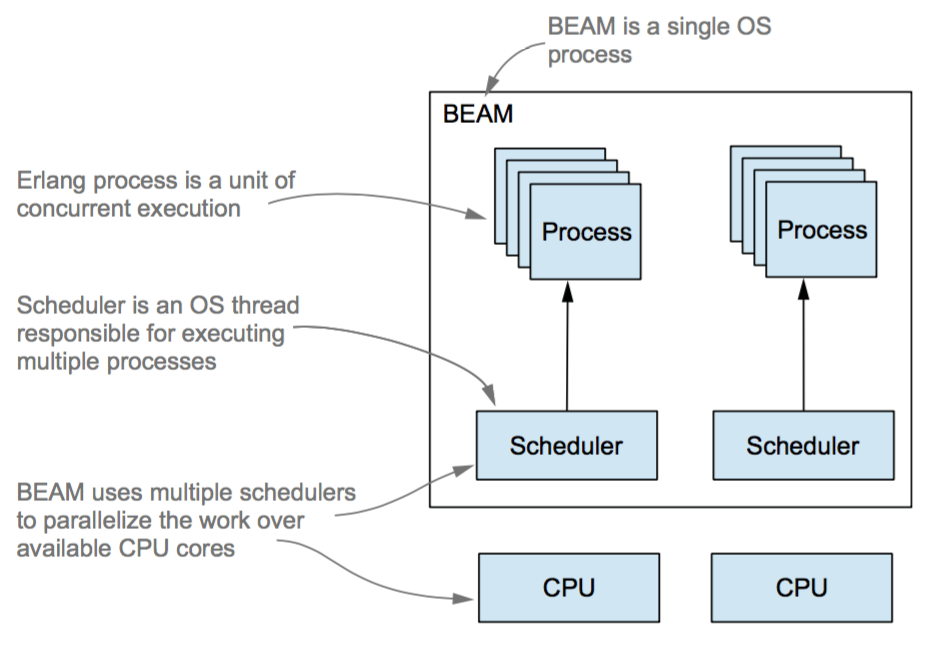
\includegraphics[scale=.5]{beam.png}
  \end{center}
\end{frame}

\begin{frame}
  \frametitle{Server side systems}
  \begin{center}
    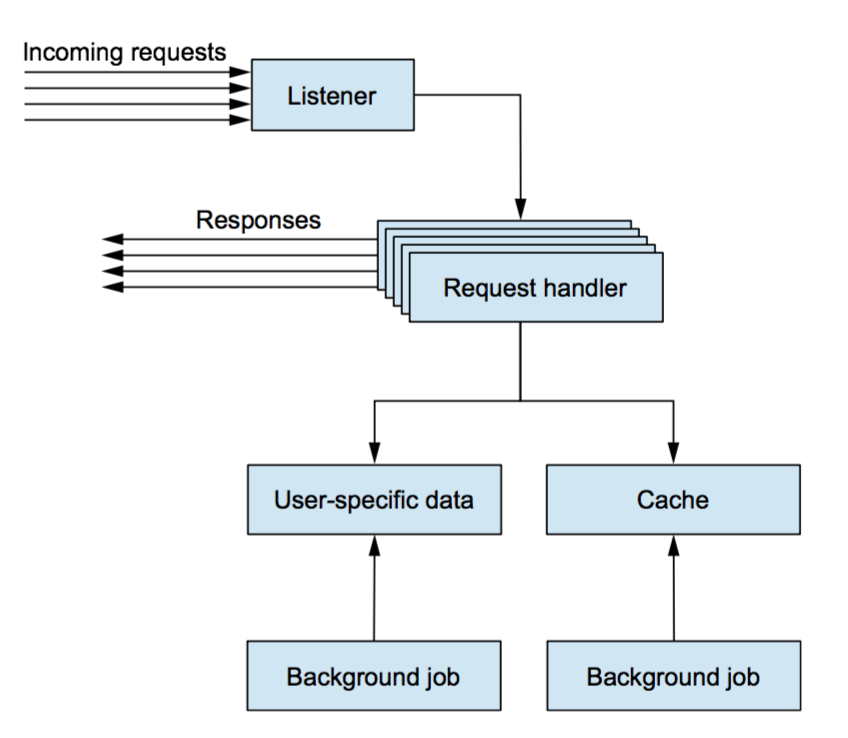
\includegraphics[scale=.5]{otp.png}
  \end{center}
\end{frame}

\begin{frame}
  \frametitle{A modern system}
  \begin{center}
    \begin{tabular}{c|c}
      \hline
      Technical requirements & Server \\ \hline
      HTTP server & Nginx and Phusion Passenger \\
      Request processing & Ruby on Rails \\
      Long-running requests & Java and Go \\
      Server-wide state & Redis \\
      Persistable data & Redis and MongoDB \\
      Background jobs & Cron, Bash scripts, and Ruby \\
      Service crash recovery & Upstart \\
      \hline
    \end{tabular}
  \end{center}
\end{frame}

\begin{frame}
  \frametitle{OTP}
  \begin{center}
    \begin{tabular}{c|c}
      \hline
      Technical requirements & Server \\ \hline
      HTTP server & Erlang \\
      Request processing & Erlang \\
      Long-running requests & Erlang \\
      Server-wide state & Erlang \\
      Persistable data & Erlang \\
      Background jobs & Erlang \\
      Service crash recovery & Erlang \\
      \hline
    \end{tabular}
  \end{center}
\end{frame}

\section[Section]{Elixir basics}

\begin{frame}
  \frametitle{Syntax}
  \begin{quote}
  Elixir syntax is like a marriage of DSL
  friendly Ruby and the powerful hygenic macros of Clojure.
  \end{quote}
  \emph{-- Devin Torres}
\end{frame}

\begin{frame}[fragile]
  \frametitle{The basics you know}
  \begin{lstlisting}
    1 + 1           # => 2
    2 * (3 + 1) / 4 # => 2.0
    1 + 2; 1 + 3    # => 4

    greeting = "Hello World!"
    IO.puts(greeting)
    # => Hello World!
    # => :ok
  \end{lstlisting}
\end{frame}

\begin{frame}[fragile]
  \frametitle{Modules and function, oh my!}
  \begin{lstlisting}
    defmodule Geometry do
      def rectangle_area(a, b) do
        a * b
      end
    end
  \end{lstlisting}
\end{frame}

\begin{frame}[fragile]
  \frametitle{Composing functions}
  \begin{lstlisting}
    def process_xml(model, xml) do
      model
      |> update(xml)
      |> process_changes
      |> persist
    end
  \end{lstlisting}
\end{frame}

\begin{frame}[fragile]
  \frametitle{Function arity}
  \begin{lstlisting}
    defmodule Rectangle do
      def area(a), do: area(a, a)
      def area(a, b), do: a * b
    end
  \end{lstlisting}
\end{frame}

\begin{frame}[fragile]
  \frametitle{Destructuring}
  \begin{lstlisting}
    def do_something({:ok, value}) do
      # use the value here
    end

    def do_something({:warning, value}) do
      # warn user before proceeding
    end

    def do_something({:error, message}) do
      # produce a nice error message to the user
    end
  \end{lstlisting}
\end{frame}

\begin{frame}[fragile]
  \frametitle{Typespec}
  \begin{lstlisting}
    defmodule Circle do
      @pi 3.14159

      @spec area(number) :: number
      def area(r), do: r * r * @pi
        
      @spec circumference(number) :: number
      def circumference(r), do: 2 * r * @pi
    end
  \end{lstlisting}
\end{frame}

\section[Section]{Macros}

\begin{frame}
  \frametitle{Macros}
  \begin{quote}
    Lisp traditionally empowered developers because you can eliminate anything
    that's tedious through macros, and that power is really what people
    keep going back for.
  \end{quote}
  \emph{-- Rich Hickey}
\end{frame}

\begin{frame}
  \frametitle{Macros}
  \begin{itemize}
  \item code transformation at compile time
  \item code that can change semantics of the input
  \item a lot of elixir functionality is implemented in macros \textsl{e.g. def, unless}
  \item should be used sparingly
  \end{itemize}
\end{frame}

\begin{frame}[fragile]
  \frametitle{Macro expension}
  \begin{columns}
    \column {.5\textwidth}
    \begin{lstlisting}
      unless some_exp do
        block_1
      else
        block_2
      end
    \end{lstlisting}
    \column {.5\textwidth}
    \begin{lstlisting}
      if some_exp do
        block_2
      else
        block_1
      end
    \end{lstlisting}
  \end{columns}
\end{frame}

\begin{frame}[fragile]
  \frametitle{Quoting}
  \begin{lstlisting}
    quote do: sum [1, 2, 3]
    # => { :sum, [], [1, 2, 3] }

    quote do: 1 + 1
    # => { :+,
    #      [context: Elixir, import: Kernal],
    #      [1, 1] }
  \end{lstlisting}
\end{frame}

\begin{frame}[fragile]
  \frametitle{Simple macro}
  \begin{lstlisting}
    defmacro match?(left, right) do
      quote do
        case unquote(right) do
          unquote(left) ->
            true
          _ ->
            false
        end
      end
    end
  \end{lstlisting}
\end{frame}

\begin{frame}[fragile]
  \frametitle{Usine our new macro!}
  \begin{lstlisting}
    list = [{:a,1},{:b,2},{:a,3}]
    # => [a: 1, b: 2, a: 3]

    Enum.filter list, fn (thing) do
      match?({:a, _}, thing)
    end
    # => [a: 1, a: 3]

    Enum.filter list, match?({:a, _}, &1)
    # => [a: 1, a: 3]
  \end{lstlisting}
\end{frame}

\section[Section]{Tooling}

\begin{frame}
  \frametitle{IEx}
  \begin{itemize}
  \item full REPL
  \item easy to load and interact
  \item full coloring support
  \item easy extensible with user defined helpers
  \end{itemize}
\end{frame}

\begin{frame}[fragile]
  \frametitle{doctest}
  \begin{verbatim}
    @doc """
    Check if the given argument is nil or not.
    Allowed in guard clauses.

    ## Examples

      iex> nil?(1)
      false
      iex> nil?(nil)
      true
    """
  \end{verbatim}
\end{frame}


\begin{frame}
  \frametitle{Mix}
  \begin{itemize}
  \item Great build and deploy tool
  \item Based around Mix.Tasks
    \begin{itemize}
    \item Simply define run/1
    \item Easy documentation
    \item Access to 15 helper methods
    \end{itemize}
  \item Great documentation
  \end{itemize}
\end{frame}

\begin{frame}[fragile]
  \frametitle{Mix tasks}
  \footnotesize{
\begin{verbatim}
    mix clean           # Clean generated application files
    mix compile         # Compile source files
    mix deps            # List dependencies and their status
    mix deps.clean      # Remove dependencies files
    mix deps.compile    # Compile dependencies
    mix deps.get        # Get all out of date dependencies
    mix deps.unlock     # Unlock the given dependencies
    mix deps.update     # Update dependencies
    mix do              # Executes the commands separated by comma
    mix escriptize      # Generates an escript for the project
    mix help            # Print help information for tasks
    mix local           # List local tasks
    mix local.install   # Install a task locally
    mix local.rebar     # Install rebar locally
    mix local.uninstall # Uninstall local tasks
    mix new             # Creates a new Elixir project
    mix run             # Run the given expression
    mix test            # Run a project's tests
\end{verbatim}
  }
\end{frame}

\begin{frame}
  \frametitle{Hex}
  \begin{itemize}
  \item Easy to use package manager
  \item Searchable
  \item Manages dependencies
  \item Almost 2300 packages available
  \end{itemize}
\end{frame}

\begin{frame}[fragile]
  \frametitle{Iteroperability with Erlang}
  \begin{lstlisting}
    # Elixir map function
    Enum.map

    # Erlang map function
    :list.map
  \end{lstlisting}
\end{frame}
\end{document}
